\documentclass{scrartcl}
\usepackage{geometry}
\usepackage{pdfpages}[total={8.5in,11in}]
\usepackage{amssymb}
\usepackage{enumitem}
\usepackage{karnaugh-map}
\usepackage{graphicx}
\begin{document}


\begin{Large}
\begin{center}
Ulvi Bajarani
Student ID 20539914
\end{center}

\newpage
Simplify the boolean function of boolean variable specified below and draw the corresponding digital circuit of the simplified function.\\

F(a, b, c)=!a b c + a !b c +a b c\\


Concepts in practice: Digital Logic.\\



---------------o----------o---------------

Due date: 10/07/2019 (mm/dd/yyyy)

Files to be used:

Files to be delivered: homework\_04.pdf

\newpage

Let’s try to create the Karnaugh Map for the function $F(a, b, c)= \neg a * b * c + a * \neg b * c + a * b * c$ :


\begin{karnaugh-map}[4][2][1][$A, B$][$C$]\end{karnaugh-map}

Revising that the function receives 1 in cases

\begin{enumerate}[label=\alph*)]

\item a=1, b=1, c=1,
\item a=1, b=0, c=1 and
\item a=0, b=1, c=1,

\end{enumerate}

we can fill in the table like this:

\begin{karnaugh-map}[4][2][1][$A, B$][$C$]
\manualterms{0,0,0,1,0,1,0,1}
\end{karnaugh-map}

If 1 values are neighbours from either horizontal or vertical side, we can count them as clusters:

\begin{karnaugh-map}[4][2][1][$A, B$][$C$]
\manualterms{0,0,0,1,0,1,0,1}
\implicant{3}{7}
\implicant{5}{7}
\end{karnaugh-map}

It helps to simplify the functions from\\

$F(a, b, c)= \neg a * b * c + a * \neg b * c + a * b * c$\\

to\\

$F(a, b, c)= b * c + a * c = c * (b + a)$\\

There are two possible circuit implementations for this function:\\

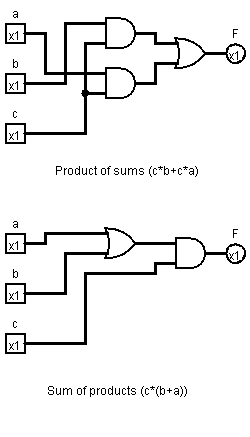
\includegraphics[scale=0.65]{Circuits.png}
\end{Large}

\end{document}